\documentclass[11pt,wide,leqno]{article}

\usepackage[utf8]{inputenc}
\usepackage[OT4, plmath]{polski}

\usepackage{lipsum}
\usepackage{mathtools}
\usepackage{amsmath}
\usepackage{amsfonts}
\usepackage{amsthm}
\usepackage[justification=centering]{caption}
\usepackage[hidelinks]{hyperref}
\usepackage{multirow}
\usepackage{titlesec}
\usepackage[dvipsnames]{xcolor}
\usepackage{pgfplots}
\usepackage[inkscapeformat=png]{svg}
\pgfplotsset{width=10cm,compat=1.9}

\usepackage[a4paper, total={6in, 8in}]{geometry}
\usepackage[justification=centering]{caption}

\newtheorem{theorem}{Twierdzenie}
\newtheorem*{fact}{Fakt}

\DeclareCaptionFormat{custom}{\texttt{#1#2}{#3}}
\captionsetup{format=custom}

\title{\textbf{Pracownia z Analizy Numerycznej (M)} \\
        Sprawozdanie do zadania \textbf{P2.7} \\}
\date{Wrocław, \today}
\author{Mateusz Łuczyński}

\begin{document}
    \maketitle
    \thispagestyle{empty}
    \titlelabel{\thetitle.\quad}
    \section{Wstęp}
        Jak powszechnie wiadomo, całkowanie znajduje swoje zastosowanie w wielu dziedzinach.
        Przydaje się ono przykładowo do liczenia pola oraz objętości pod wykresem funkcji, wyliczania długości łuków lub
        chociażby w kinematyce, do znajdywania wielkości opisujących fizyczne obiekty.
        Całkować można mnóstwo funkcji, czasem takich, o których wiadomo stosusnkowo bardzo mało.
        Sprawozdanie to zostanie poswięcone numerycznym sposobom przybliżania całek oznaczonych \(\int_{a}^{b} f(x)\,dx\)
        przy założeniu, że o funkcji podcałkowej wiemy jedynie jakie wartości przyjmuje
        w zadanych z góry punktach \(a = t_0 < t_1 < \cdots < t_n = b\).

        Rozważać będziemy trzy funkcje podcałkowe, mianowicie znaną w kontekście interpolacji wielomianowej
        funkcję Rungego \(\frac{1}{1 + 25x^2}\) na przedziale \(\left[-1,1\right]\), funkcję trygonometryczną \(\sin x\) na przedziale \(\left[0,2\pi\right]\), a także
        prosty wielomian \(2x^3 - x^2 + 3x - 7\) na przedziale \(\left[-3,3\right]\). Wykresy tych funkcji w podanych zakresach
        znajdują się odpowiednio na rysunkach~\ref{runge},~\ref{sin} oraz~\ref{rzulty}.

        Użyte algorytmy wraz z testami numerycznymi znaleźć można w pliku \texttt{program.jl} 
        (lub w wersji interaktywnej w pliku \texttt{program.ipynb}) załączonym do 
        sprawozdania. 
        
        \begin{figure}[h]
            \begin{minipage}{0.5\linewidth}
                \centering
                \begin{tikzpicture}[scale=0.7]
                    \begin{axis}[
                        axis lines = left,
                        xtick = {-1,-0.5,0,0.5,1},
                        ytick = {0.2, 0.4, 0.6, 0.8, 1}
                    ]
                        \addplot[
                            domain=-1:1,
                            samples=100]
                            {1/(1+25*x^2)};
                    \end{axis}
                \end{tikzpicture}
                \vspace*{-3mm}\caption{Funkcja Rungego}\label{runge}
            \end{minipage}\hfill
            \begin{minipage}{0.5\linewidth}
                \centering
                \begin{tikzpicture}[scale=0.7]
                    \begin{axis}[
                        axis x line shift = -1,
                        axis lines = left,
                        xtick = {pi/2, pi, 3*pi/2, 2*pi},
                        xticklabels = {\(\frac{\pi}{2}\), \(\pi\), \(\frac{3\pi}{2}\), \(2\pi\)}
                    ]
                        \addplot[
                            domain=0:2*pi,
                            samples=100]
                            {sin(deg(x))};
                    \end{axis}
                \end{tikzpicture}
                \vspace*{-3mm}\caption{\(f(x) = \sin x\)}\label{sin}
            \end{minipage}\vspace{0.5cm}
        \end{figure}

        \begin{figure}
            \begin{minipage}{\linewidth}
                \centering
                \begin{tikzpicture}[scale=0.7]
                    \begin{axis}[
                        axis lines = left,
                        axis x line shift = -79
                    ]
                        \addplot[
                            domain=-3:3,
                            samples=100]
                            {2*x^3 - x^2 + 3*x - 7};
                    \end{axis}
                \end{tikzpicture}
                \vspace*{-3mm}\caption{Wielomian \(2x^3 - x^2 + 3x - 7\)}\label{rzulty}
            \end{minipage}
        \end{figure}

    \section{Sposób pierwszy}
        Jednym ze sposobów przybliżenia całki z zadanej funkcji
        jest scałkowanie wielomianu interpolującego tą funkcję w podanych punktach. 
        Takie całkowanie można wtedy wykonać w sposób zmechanizowany, mianowicie dla wielomianu \(p(x)\)
        w postaci potęgowej zachodzi następujący wzór
        \begin{equation}
            P(x) := \int p(x)\,dx = \int \sum_{i=0}^{n} a_i x^i \,dx =
            c + \sum_{i=1}^{n+1} \frac{a_{i-1}}{i} x^{i}, \quad c = \text{const}
        \end{equation}
        Oczywiście w przypadku liczenia całki oznaczonej stała \(c\) redukuje się i pozostaje nam
        policzyć różnicę \(P(b) - P(a)\) (korzystając przykładowo dwukrotnie ze schematu Hornera).
        Wynik całkowania w ten sposób powinien zatem zależeć głównie od tego jak dobrze uda się 
        zinterpolować daną funkcję.

        W załączonych testach numerycznych dla każdej funkcji wspomnianej we wstępie najpierw podzielono rozważane przedziały na podprzedziały równej długości, potem wylosowano w nich
        zestaw \(n\) punktów (dla różnych \(n\)), następnie wyznaczono postać Newtona wielomianu interpolującego daną funkcję w 
        wylosowanych punktach, żeby na końcu scałkować ten wielomian sprowadzony do postaci potęgowej.

        Na rysunku~\ref{sininter} czerwoną linią zaznaczono wielomian interpolacyjny 4-tego stopnia dla funkcji \(\sin x\). 
        \begin{figure}[h]
            \begin{minipage}{0.5\linewidth}
                \centering
                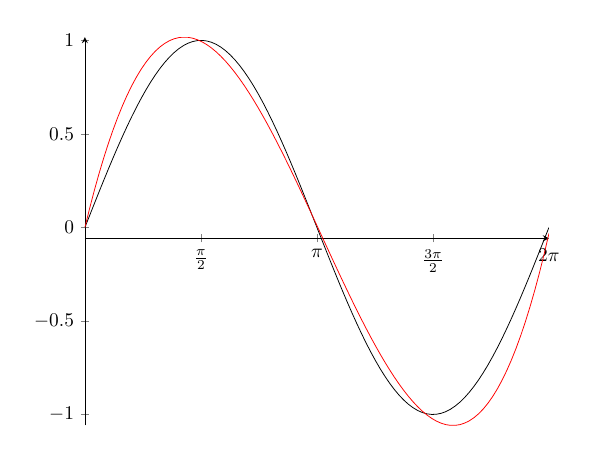
\begin{tikzpicture}[scale=0.7]
                    \begin{axis}[
                        axis x line shift = -1,
                        axis lines = left,
                        xtick = {pi/2, pi, 3*pi/2, 2*pi},
                        xticklabels = {\(\frac{\pi}{2}\), \(\pi\), \(\frac{3\pi}{2}\), \(2\pi\)}
                    ]
                        \addplot[
                            domain=0:2*pi,
                            samples=100]
                            {sin(deg(x))};
                        \addplot[
                            domain=0:2*pi,
                            samples=100,
                            color=red
                        ]{0.0000+1.6503*x^1-0.7654*x^2+0.0736*x^3+0.0010*x^4};
                    \end{axis}
                \end{tikzpicture}
                \vspace*{-3mm}\caption{Interpolacja \(\sin x\) wielomianem 4-tego stopnia}\label{sininter}
            \end{minipage}\hfill
            \begin{minipage}{0.5\linewidth}
                \centering
                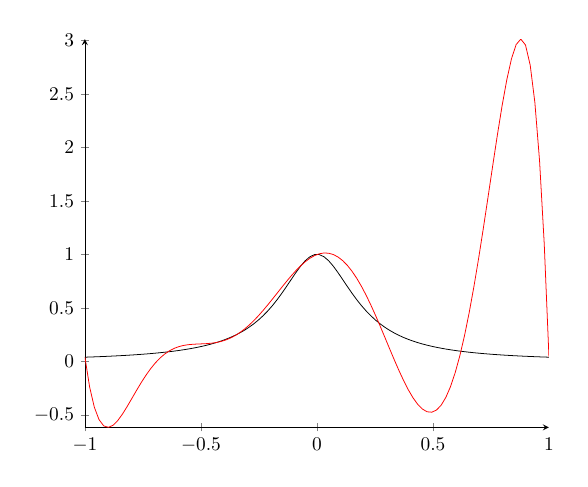
\begin{tikzpicture}[scale=0.7]
                    \begin{axis}[
                        axis lines = left,
                        xtick = {-1,-0.5,0,0.5,1},
                    ]
                        \addplot[
                            domain=-1:1,
                            samples=100]
                            {1/(1+25*x^2)};
                        \addplot [
                            domain=-1:1,
                            samples=100,
                            color=red]
                            {0.9978+0.8300*x^1-10.7450*x^2-15.8275*x^3+29.4528*x^4+48.1457*x^5-19.6673*x^6-33.1481*x^7};
                    \end{axis}
                \end{tikzpicture}
                \vspace*{-3mm}\caption{Interpolacja funkcji Rungego wielomianem 7 stopnia}\label{rungeinte}
            \end{minipage}
        \end{figure}
        Jak widać na wykresie wyznaczony wielomian zadany wzorem
        \begin{equation}
            P_1(x) = 1.6503x^1 - 0.7654x^2 + 0.0736x^3 + 0.0010x^4
        \end{equation}
        wygląda na satysfakcjonujące przybliżenie funkcji sinus. Można się zatem spodziewać, że i szukana całka będzie całkiem bliska rzeczywistości.
        Obliczając \(\int_{0}^{2\pi} P_1(x)\,dx\) otrzymujemy wartość \(-0.07449912033229149\). Porównując wynik 
        z faktyczną wartością \(\int_{0}^{2\pi} \sin x \,dx = 0\) widać, że otrzymaliśmy
        przybliżenie na poziomie dwóch cyfr dokładnych. Wynik zachowuje się w podobny sposób również wtedy, kiedy
        \(n \leq 7\). Dla większych wartości \(n\) błąd wyznaczania współczynników potęgowej postaci wielomianu
        interpolacyjnego zaczyna być bardzo zauważalny, co powoduje dosadny spadek dokładności wyniku. Można zatem dojść do wniosku, że 
        w celu zmaksymalizowania wydajności metody, powinno się korzystać z niezbyt dużej ilości punktów węzłowych.

        Dla wielomianu \(2x^3 - x^2 + 3x - 7\) i takiej samej wartości \(n\) jak w przypadku pierwszego podejścia do liczenia całki z \(\sin x\) metoda działa bez zarzutów
        (wielomianem interpolującym będzie ten sam wielomian, zatem całkować będziemy dokładnie tą samą funkcje).
        Zmiana wartości \(n\) nie wpływa na skuteczność liczenia całki. Można zatem stwierdzić, że metoda idealnie sprawdza się w sytuacjach
        gdzie rozpatrywana funkcja jest wielomianem.

        W przypadku funkcji Rungego interpolacja jest bardzo niedokładna, niezależnie od wyboru \(n\) (przykładowy 
        wielomian interpolacyjny dla \(n=8\) zaznaczono na rysunku~\ref{rungeinte}).
        Wynika to głównie z faktu, że nie mamy wpływu na wybór punktów węzłowych. Oczywiście powoduje to 
        praktycznie losową dokładność wyniku obliczenia całki, przykładowo w przykładzie z 
        rysunku~\ref{rungeinte} całka wynosi \(0.9943045091703662\), podczas gdy faktyczny wynik wynosi 
        w przybliżeniu \(\approx 0.54936\). Metoda nie sprawdza się zatem w przypadku
        niektórych bardziej problematycznych funkcji. 

        Zdecydowanymi zaletami podejścia opisanego wyżej jest prostota interpolacji oraz 
        całkowania wielomianów w postaci potęgowej. Główną wadą zaś jest niedokładność wyznaczania 
        współczynników takiego wielomianu dla dużych wartości \(n\), przez co jesteśmy skazani
        na korzystanie z małej ilości punktów węzłowych, w celu uniknięcia znacznych zaburzeń wyników.
        Kolejną wadą jest na pewno brak możliwości manipulowania doborem punktów węzłowych, przez co interpolacja jest 
        podatna na typowe efekty uboczne (takie jak efekt Rungego możliwy do zaobserwowania na rysunku~\ref{rungeinte}).

    \section{Sposób drugi}
        Inną możliwością przybliżania rozważanej całki jest metoda zwana metodą trapezów. Polega ona 
        na aproksymacji pola pod wykresem funkcji polami trapezów budowanych na przedziałach pomiędzy wylosowanymi punktami \(x_i\).
        Wizualizacja tej metody znajduje się na rysunku~\ref{trapezy}.

        \begin{figure}[h]
            \centering
            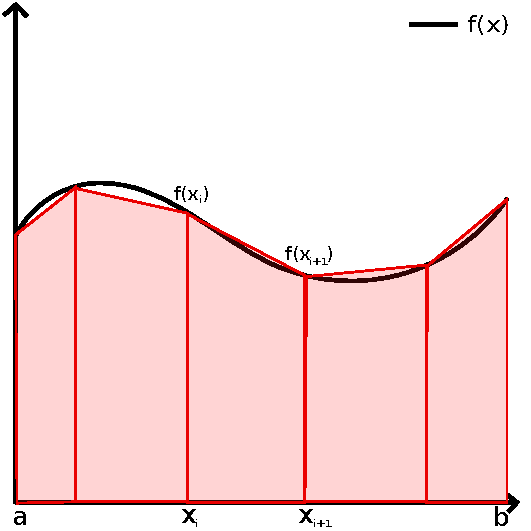
\includegraphics[scale=0.75]{../prog/bitmap.pdf}
            \caption{Wizualizacja metody trapezów. Całkę \(\int_{a}^{b} f(x)\,dx\) przybliżamy sumą
            pól czerwonych trapezów}\label{trapezy}
        \end{figure}

        Dla wylosowanych punktów \(x_i\) wzór na przybliżoną całkę z funkcji o stałym znaku wyraża się w następujący sposób
        \begin{equation}
            \int_{a}^{b} f(x)\,dx \approx \sum_{i=0}^{n} \frac{(f(x_i) + f(x_{i+1}))(x_{i+1}-x_i)}{2}
        \end{equation}
        W przypadku funkcji przyjmującej na zmianę wartości ujemne i dodatnie trzeba dodatkowo pilnować
        znaków składników sumy i zastępować niektóre trapezy dwoma trójkątami.

        Testy ponownie przeprowadzono losując punkty w przedziałach o równej długości dla trzech funkcji:
        \(\sin x, \frac{1}{1+25x^2}\) oraz \(2x^3 - x^2 + 3x - 7\).
        Dla funkcji Rungego i \(n=100\) wynik jest bardzo satysfakcjonujący, gdyż wynosi \(0.549399\)
        (dokładny wynik wynosi \(\approx 0.54936\)). Ponowne testy dla tej samej wartości \(n\)
        za każdym razem zwracają wynik na tym samym poziomie. Dla mniejszych wartości \(n\) natomiast 
        zauważalny jest spadek dokładności wyników. Dla \(n=5\) wacha się on z reguły w okolicach
        \(0.4\) oraz \(0.6\). W przypadku funkcji \(\sin x\) sytuacja wygląda podobnie, gdyż dla małych \(n\)
        błąd bezwzględny wyniku sięga wartości równych \(\approx 1\), czego nie da się powiedzieć o błędzie dla \(n\) znacznie większych.
        Przykładowo znowu dla \(n\) równego \(100\) całka \(\int_{0}^{2\pi}\ \sin x\,dx\) oblicza się do wartości rzędu 
        \(10^{-5}\), co jest bardzo dobrym wynikiem (widać tutaj przy okazji przewage tej metody nad metodą wykorzystującą interpolacje, w tym konkretnym przypadku).
        Całkując tą metodą wielomian \(2x^3 - x^2 + 3x - 7\) można ponownie zauważyć
        spadek efektywności metody dla małej ilości punktów \(x_i\), co nie występywało w przypadku interpolacji, gdzie wynik 
        był praktycznie dokładny dla dowolnej wartości \(n\).

        Ogólnie można dojśc do wniosków, że metoda trapezów wydaje się całkiem efektywną metodą w przypadku,
        gdy mamy do dyspozycji wiedzę o wartościach funkcji w dużej ilości punktów. Jej zaletą jest również 
        prostota implementacji i prosty w zrozumieniu koncept, który pomimo to jest w stanie wyprodukować
        bardzo dobre wyniki. Nie sprawdza się ona jednak w momencie, gdy znanych punktów jest bardzo mało lub gdy 
        wartości funkcji w przedziałach pomiędzy wylosowanymi punktami momentalnie eksplodują, żeby następnie wrócić
        do liczb rzędu takiego jak przed skokiem. 

    \section{Konkluzja}
        W sprawozdaniu przedstawione zostały dwie metody przybliżania całki \(\int_{a}^{b} f(x)\,dx\) znając jedynie wartości funkcji 
        podcałkowej w z góry zadanych punktach z przedzialu \([a,b]\). Testy numeryczne wykazały, że obie te metody posiadają zarówno swoje 
        wady jak i zalety. 
        
        Metoda wykorzystująca interpolacje podatna jest na efekty uboczne takie jak efekt Rungego, oraz 
        błędy wyznaczania postaci potęgowej wielomianu. Nie mniej jednak wyniki dla niektórych typów funkcji uzyskane tą metodą 
        wydają się satysfakcjonujące zważając na małą ilość informacji o funkcji podcałkowej. Jest ona również zdecydowanie lepsza od drugiej metody
        w przypadku, kiedy mamy do czynienia z mała ilością punktów \(x_i\).  

        Z drugiej strony, w momencie kiedy dysponujemy dużą ilością znanych wartości funkcji \(f\)
        lepszym wyborem okazuje się metoda trapezów, która prezentuje wyniki o znacznie zwiększonej dokładności dla dużych wartości \(n\).
        Również ona jednak nie jest pozbawiona swoich wad. Niefortunne ułożenie znanych wartości funkcji może doprowadzić do 
        ogromnych błędów aprosymacji. 
        
        Analizując wady obu tych metod można zauważyć istote doboru odpowiednich punktów używanych do obliczania kwadratur 
        funkcji. Bardziej zaawansowane metody przybliżania całek, mające dostęp do manipulowania wyborem ciągu \(x_i\), pozbywają się 
        większości problemów omówionych w sprawozdaniu. Obliczając całki, znając tylko losowe jej wartości, trzeba 
        liczyć się zatem z nieuniknionym spadkiem dokładności.



\end{document}
